%!TEX root = Thesis.tex

\chapter{Experimental}
\label{ch:expt}

\section{General procedures}
\label{section:generalprocedures}

\fixme{copied from Almas, check that the necessary info is here, everything is correct and everything unneccessary is removed}

All reactions and manipulation of products and reagents were carried out under an inert nitrogen atmosphere using standard Schlenk line techniques unless otherwise stated.  Analytical grade reagents and high purity solvents were degassed and purged with nitrogen before use, except for diethyl ether and tetrahydrofuran which were dried by refluxing over sodium/benzophenone ketyl.  NMR spectra were recorded using a Varian Unity Inova 300 (300~MHz for \proton, 75~MHz for \carbon, 121~MHz for \phosphorus{} and 282~MHz for \fluorine), a Varian Unity Inova 500 (500~MHz for \proton{} and 125~MHz for \carbon), or a Varian DirectDrive 600 (600~MHz for \proton and 150~MHz for \carbon{}) spectrometers.   The 600~MHz instrument was equipped with a Varian inverse-detected triple-resonance HCN cold probe operating at 25~K.  All direct-detected \proton{} and \carbon{} chemical shifts were referenced to the residual solvent peak.\cite{Fulmer2010}  NMR samples were prepared under an inert nitrogen or argon atmosphere unless otherwise stated, using \ce{C6D6}, \ce{CDCl3}, \ce{CD2Cl2}, acetone-\ce{d6} and toluene-\ce{d8}.  All NMR solvents were degassed before use and stored under inert atmosphere over molecular sieves.  Variable temperature NMR was carried out in toluene-\ce{d8} or \ce{CD2Cl2} using Varian Unity Inova 300~MHz NMR spectrometer.  Infrared spectra were recorded with a PerkinElmer Spectrum One FT-IR spectrophotometer using pressed KBr discs.  Microanalyses were performed by The Campbell Microanalytical Laboratory at Otago University.  Melting points were recorded on a Gallenkamp Melting Point Apparatus under vacuum unless otherwise stated. Single crystal \textit{X}-ray diffraction data were recorded by the \textit{X}-ray Crystallography Laboratory at the University of Canterbury.  Electrospray ionisation mass spectra were either recorded on a PE Biosystem Mariner 5158 TOF mass spectrometer at Victoria University, or performed by the GlycoSyn QC laboratory at Industrial Research Limited using a Waters Q-TOF Premier Tandem mass spectrometer.  Calculated \proton{} NMR spectra were obtained from gNMR spectral simulation programme, version 5.0.6.0 written by P. H. M. Budzelaar, IvorySoft 2006.

%\subsection*{Crystallography} 
%\label{subsec:X-ray}

%Diffraction data\footnote{Bruker {\scriptsize{SMART}} (Version 5.054), {\scriptsize{SADABS}} (Version 2.03), and {\scriptsize{SAINT}} (Version 6.02A), Bruker AXS Inc., Madison, Wisconsin, USA, 1997.} (see Tables \ref{tab:dataPN582}, \ref{tab:dataPdPNCl2}, \ref{tab:datanbagostic}, \ref{tab:datadimer} for details) were collected using Bruker CCD diffractometers with Mo K$\alpha$ radiation (0.71073~\AA) from fine-focus sealed tubes with graphite monochromators, using phi and omega scans.  Multi-scan absorption corrections were applied.  The structures were solved by direct methods and full-matrix least squares refinement,\footnote{G. M. Sheldrick, {\scriptsize{SHELX-97}}.  Programmes for the Solution and Refinement of Crystal Structures, 1997.} with anisotropic thermal parameters for all non-H atoms.\cite{Sheldrick}  Hydrogen atoms are in calculated positions and refined using a riding model with {\scriptsize{SHELXL}} defaults.  The agostic hydrogen atom in \ce{Pt-H-C} interaction was located and its position refined, and all relevant bond distances and angles were calculated using Mercury, version 1.4.2.  Molecular drawings were made using ORTEP3.\cite{ORTEP}

\section{Ligands and Non-Transition Metal Derivatives}
\label{section:experimental:ligands}

%%%%%
%S-tBu %
%%%%%
%\newpage{}
\subsection*{2,8-Dimethyl-4,6-bis(di-\emph{tert}-butylphosphino)phenoxathiin \\(\emph{t}-Bu-thixantphos)}

\begin{structure}
\begin{center}
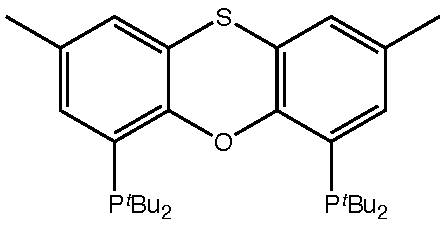
\includegraphics[scale=0.7]{../Structures/SP(tBu)2_ligand.pdf}
\end{center}
\end{structure}

\noindent{}\emph{s}-Butyllithium (29.8 mL, 1.0 M in cyclohexane, 29.8 mmol) was added dropwise to a stirred solution of 2,8-dimethylphenoxathiin (2.27 g, 9.94 mmol) and TMEDA (4.47 mL, 29.8 mmol) in diethyl ether (96 mL) at -78\degC{}.  The resulting yellow solution was warmed to at room temperature and stirred for a further 16 hours over which time a dark red colour developed.  The reaction was cooled to -78\degC{} and chlorodi-\emph{t}-butylphosphine (5.67 mL, 29.8 mmil) was added dropwise.  The reaction mixture was stirred for a further seven days resulting in a yellow solution with a white precipitate of lithium chloride.  The solvent was removed \emph{in vacuo} giving an orange oil.  This oil was taken up in dichloromethane (25 mL) and washed with water (3 x 15 mL).  The organic layer was passed through a column of magnesium sulfate and solvent was removed \emph{in vacuo}.  The product was purified by dissolving in hot \emph{n}-propanol and cooling at \fixme{temperature} giving small white crystals (1.33 g, 26\%).  This compound can be handled in the air for short periods however, should be stored under an inert atmosphere.
\Phosphorusintro{CDCl3}
\NMRPsinglet{9.5}.
\Protonintro{500}{\fixme{CDCl3}}
\NMRsinglet{7.29}{PC(Ar)C\emph{H}},
\NMRsinglet{6.88}{SCC\emph{H}},
\NMRsinglet{2.25}{C(Ar)\ce{C\emph{H}3}},
\NMRmultiplet{1.22-1.24}{PCC\emph{H}\textsubscript{3}}.
\Carbonintro{125}{\fixme{CDCl3}}
\NMRPC{155.3}{vt}{13.0}{\emph{C}O}
\NMRsinglet{134.6}{PC(Ar)\emph{C}H}
\NMRsinglet{131.9}{SCC\emph{C}(\ce{CH3})}
\fixme{something at 128?}
\NMRsinglet{127.4}{SC\emph{C}H}
\NMRPC{120.1}{vt}{2.4}{\emph{C}S}
\fixme{tBu groups}
\NMRPC{30.8}{vt}{9.1}{PC\emph{C}\ce{H3}}
\NMRsinglet{20.9}{C(Ar)\emph{C}\ce{H3}}.
\fixme{IR, EA, MS}

%%%%%
%Si-tBu%
%%%%%
%\newpage{}
\subsection*{4,6-bis(di-\emph{tert}-butylphosphino)-10,10-dimethylphenoxasilin \\(\emph{t}-Bu-sixantphos)}

\begin{structure}[h]
\begin{center}
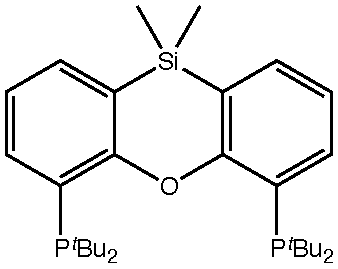
\includegraphics[scale=0.7]{../Structures/SiP(tBu)2_ligand.pdf}
\end{center}
\end{structure}

This compound was prepared similarly to \fixme{reference to S-tBu ligand} using 10,10-dimethylphenoxasilin (0.40 g, 1.8 mmol) giving white crystals (0.127 g, 14\%).
\Phosphorusintro{CD2Cl2}
\NMRPsinglet{8.42} \fixme{it has silicon satellites? should I add them?}.
\Protonintro{500}{CD2Cl2}
\NMRsinglet{0.46}{SiC\emph{H}\textsubscript{3}}
\NMRPH{1.29}{vt}{5.6}{PCC\emph{H}\textsubscript{3}}
\NMRHH{7.12}{t}{7.5}{PCCC\emph{H}}
\NMRHH{7.53}{d}{7.1}{SiCC\emph{H}}
\NMRHH{7.87}{d}{7.4}{PCC\emph{H}}.
\Carbonintro{125}{CD2Cl2}
\NMRPC{164.3}{vt}{11.3}{\emph{C}O}
\NMRsinglet{138.5}{PC\emph{C}H}
\NMRsinglet{134.8}{SiC\emph{C}H}
\NMRsinglet{\fixme{128}}{P\emph{C}(Ar)}
\NMRsinglet{121.4}{PCC\emph{C}H}
\NMRsinglet{119.4}{Si\emph{C}(Ar)}
\NMRPC{33.2}{\fixme{dd}}{16.3, 13.9}{P\emph{C}\ce{CH3}}
\NMRPC{31.0}{vt}{9.6}{PC\emph{C}\ce{H3}}
\NMRsinglet{-0.09}{Si\emph{C}\ce{H3}}.
\fixme{IR, mass spec, EA}

\fixme{change the NMR data so it goes from large to small}

%%%%%%%
%S-tBu acid%
%%%%%%%
\subsection*{Protonated 2,8-Dimethyl-4,6-bis(di-\emph{tert}-butylphosphino)phenoxathiin \\(\emph{t}-Bu-thixantphos) with \ce{CH2(SO2CF3)2}}

\begin{structure}[h]
\begin{center}
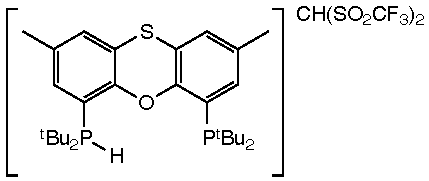
\includegraphics{../Structures/StBuH.pdf}
\end{center}
\end{structure}

%Reaction 1093
2,8-Dimethyl-4,6-bis(di-\emph{tert}-butylphosphino)phenoxathiin \\(\emph{t}-Bu-thixantphos) and \ce{CH2(SO2CF3)2} were combined in an NMR tube and dissolved in \ce{CD2Cl2}.  

\Phosphorusintro{CD2Cl2}
\NMRPsinglet{15.8}
\Protonintro{500}{CD2Cl2}
\NMRmultiplet{8.99}{P\emph{H}}
\NMRsinglet{7.29}{SCC\emph{H}},
\NMRsinglet{7.22}{PC(Ar)C\emph{H}},
\NMRsinglet{3.83}{\ce{C\emph{H}(SO2CF3)}}
\NMRsinglet{2.36}{C(Ar)\ce{C\emph{H}3}},
\NMRmultiplet{1.41-1.44}{PCC\emph{H}\textsubscript{3}}.
\Carbonintro{125}{\fixme{CD2Cl2}}
\NMRsinglet{152.9}{\emph{C}O}
\NMRsinglet{136.2}{SCC\emph{C}(\ce{CH3})}
\NMRsinglet{132.5}{SC\emph{C}H}
\NMRsinglet{131.8}{PC(Ar)\emph{C}H}
\NMRsinglet{122.2}{\emph{C}S}
\NMRCF{121.5}{quartet}{325.6}{\ce{CF3}}
\NMRsinglet{115.3}{\emph{C}(Ar)}
\NMRsinglet{34.4}{P\emph{C}C\ce{H3}}
\NMRsinglet{29.5}{PC\emph{C}\ce{H3}}
One peak (\emph{C}\ce{H(SO2CF3)}) obscured by solvent.
\fixme{IR, EA, MS}

%%%%%%%%
% Si-tBu acid %
%%%%%%%%
\subsection*{Protonated 4,6-bis(di-\emph{tert}-butylphosphino)-10,10-dimethylphenoxasilin\\(\emph{t}-Bu-Sixantphos) with \ce{CH2(SO2CF3)2}}

\begin{structure}[h]
\begin{center}
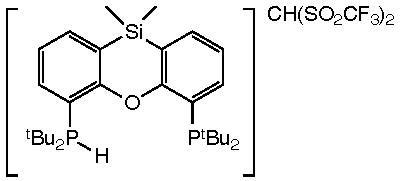
\includegraphics{../Structures/SitBuH.pdf}
\end{center}
\end{structure}

%Reaction4010\\
4,6-bis(di-\emph{tert}-butylphosphino)-10,10-dimethylphenoxasilin (\emph{t}-Bu-Sixantphos) and \ce{CH2(SO2CF3)2} were combined in an NMR tube and dissolved in \ce{CDCl3}.  

%Phosphorus
\Phosphorusintro{CDCl3}
\NMRPsinglet{14.3}
%Proton
\Protonintro{500}{CDCl3}
\NMRmultiplet{9.57}{P\emph{H}}
\NMRmultiplet{7.85-7.87}{PCC\emph{H}}
\NMRHH{7.79}{d}{6.6}{SiCC\emph{H}}
\NMRHH{7.41}{t}{7.5}{PCCC\emph{H}}
\NMRbsinglet{4.06}{C\emph{H}\ce{(SO2CF3)2}}
\NMRPH{1.43}{vt}{7.5}{PCC\emph{H}\textsubscript{3}}
\NMRsinglet{0.53}{SiC\emph{C}\ce{H3}}
%Fluorine
\Fluorineintro{CDCl3}
\NMRsinglet{-80.8}{C\emph{F}\textsubscript{3}}
%Carbon
\Carbonintro{125}{CDCl3}
\NMRPC{161.5}{vt}{5.3}{\emph{C}O}
\NMRsinglet{139.1}{SiC\emph{C}H}
\NMRsinglet{136.9}{PC\emph{C}H}
\NMRPC{124.0}{vt}{2.4}{PCC\emph{C}H}
\NMRsinglet{121.1}{Si\emph{C}(Ar)}
\NMRCF{121.1}{quartet}{327.2}{CH\ce{(SO2}\emph{C}\ce{F3)2}}
\NMRbsinglet{115.0}{P\emph{C}(Ar)}
\NMRsinglet{53.6}{\emph{C}H\ce{(SO2CF3)2}}
\NMRPC{34.2}{vt}{3.9}{P\emph{C}\ce{CH3}}
\NMRPC{29.5}{vt}{4.3}{PC\emph{C}\ce{H3}}
\NMRsinglet{-0.4}{Si\emph{C}\ce{H3}}

\fixme{IR, EA, MS}

%%%%%%
%CtBu Se%
%%%%%%

%Reaction4031
\subsection*{9,9-Dimethyl-4,6-bis(di\emph{tert}-butylphosphino)xanthene}

\begin{structure}[h]
\begin{center}
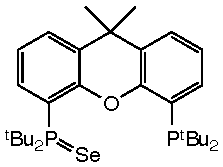
\includegraphics{../Structures/CtBuSe.pdf}
\end{center}
\end{structure}

\fixme{rewrite this}Some CtBu ligand was combined with lots of selenium in a flask under nitrogen and heated to reflux with stirring for 3 days.  After which the excess selenium was removed by filtration and the solvent was remove in vacuo to obtain a pale yellow oil with a yield in excess of 100\% due to the enormous amount of grease present.

\section{Silver Complexes}
\label{section:experimental:silver}

%%%%%%
%AgCl StBu%
%%%%%%

%Reaction3002
%\newpage{}

\subsection*{\emph{t}-Bu-thixantphossilverchloride, 3003} \fixme{check name}

\begin{structure}[h]
\begin{center}
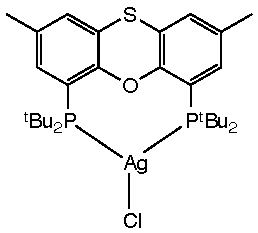
\includegraphics{../Structures/StBuSilverChloride.pdf}
\end{center}
\end{structure}

This reaction was carried out in the dark.  \fixme{StBu ligand} (88 mg, 0.17 mmol) and silver chloride (24 mg, 0.17 mmol) were combined \ce{CH2Cl2} (4 mL) in a Schlenk tube.  After 5 days stirring the solution was passed through a plug of alumina, washing with dichloromethane (4 x 1 mL).  The solvent was removed in vacuo giving a cloudy oil.  The oil was triturated with hexane (2 mL) yielding the title compound as a white powder (94 mg, 84\%).  The resulting silver complex is light sensitive and care should be taken to exclude light.

\fixme{check if in vacuo should be italicised} 

%Phosphorus
\Phosphorusintro{CDCl3}
\NMRAgP{21.81}{406.7}{469.6}.
%Proton
\Protonintro{600}{CDCl3}
\NMRPH{7.39}{d}{1.0}{PC(Ar)C\emph{H}},
\NMRPH{7.11}{d}{1.6}{SCC\emph{H}},
\NMRsinglet{2.31}{C(Ar)\ce{C\emph{H}3}}
\NMRmultiplet{1.41}{PCC\emph{H}\textsubscript{3}}.
%Carbon
\Carbonintro{150}{CDCl3}
\NMRPC{155.5}{vt}{6.6}{\emph{C}O}
\NMRPC{134.8}{d}{4.9}{PC(Ar)\emph{C}H}
\NMRPC{133.1}{d}{1.5}{\emph{C}(Ar)\ce{CH3}}
\NMRsinglet{130.3}{SC\emph{C}H})
\NMRPC{122.8}{vt}{3.0}{\emph{C}S}
\NMRmultiplet{120.9}{P\emph{C}(Ar)} \fixme{virtual quartet?}
\NMRmultiplet{35.3}{P\emph{C}C\ce{H3}} \fixme{virtual quartet?}
\NMRPC{30.9}{vt}{5.6}{PC\emph{C}\ce{H3}}
\NMRsinglet{20.8}{C(Ar)\emph{C}\ce{H3}}
\fixme{IR, EA, MS}
\fixme{Check frequency of 13C on 600 MHz}

%%%%%%%%
% AgCl SitBu %
%%%%%%%%

%Reaction3003
%\newpage{}
\subsection*{\emph{t}-Bu-Sixantphossilverchloride} \fixme{check name}
\begin{structure}[h]
\begin{center}
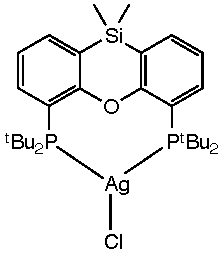
\includegraphics{../Structures/SitBuSilverChloride.pdf}
\end{center}
\end{structure}

This reaction was carried out in the dark.  Combined \fixme{SitBu ligand} and silver chloride in an NMR tube and dissolved in \ce{CDCl3} and sonicated for 5 mins.  After four days the reaction was sonicated for 6 x 5 mins.  Decanted the solution and washed the solid with dichloromethane (3 x 1 mL).  The solution was removed in vacuo yielding the title compound as a white solid (31 mg, 97\%).  The resulting silver complex is light sensitive and care should be taken to exclude light.

%Phosphorus
\Phosphorusintro{CDCl3}
\NMRAgP{24.2}{408.1}{471.1}
%Proton
\Protonintro{600}{CDCl3}
\NMRmultiplet{7.88}{PCC\emph{H}}
\NMRdd{7.61}{7.0}{1.8}{SiCC\emph{H}}
\NMRHH{7.21}{t}{7.3}{PCCC\emph{H}}
\NMRmultiplet{1.42}{PCC\emph{H}\textsubscript{3}}
\NMRsinglet{0.46}{SiC\emph{H}\textsubscript{3}}
%Carbon
\Carbonintro{150}{CDCl3}
\NMRPC{163.9}{vt}{5.2}{\emph{C}O}
\NMRPC{138.2}{d}{4.4}{PC\emph{C}H}
\NMRsinglet{136.3}{SiC\emph{C}H}
\NMRsinglet{122.2}{Si\emph{C}(Ar)}
\NMRsinglet{122.1}{PCC\emph{C}H}
\NMRmultiplet{120.5}{P\emph{C}(Ar)} \fixme{quartet?}
\NMRmultiplet{35.5}{P\emph{C}\ce{CH3}} \fixme{quartet?}
\NMRPC{31.0}{vt}{5.6}{PC\emph{C}\ce{H3}}
\NMRsinglet{-1.3}{Si\emph{C}\ce{H3}}.
\fixme{IR, mass spec, EA}


%%%%%%%
%AgCl CtBu%
%%%%%%%

%Reaction3017
%\newpage{}
\subsection*{\emph{t}-Bu-xantphossilverchloride} \fixme{check name}

\begin{structure}[h]
\begin{center}
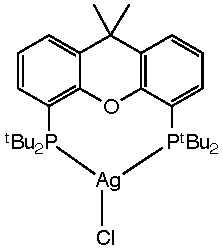
\includegraphics{../Structures/CtBuSilverChloride.pdf}
\end{center}
\end{structure}

This reaction was carried out in the dark as silver chloride and the product are light sensitive.  Combined \fixme{CtBu ligand} (17 mg, 0.034 mmol) and silver chloride (5 mg, 0.035 mmol) in an NMR tube and dissolved in \ce{CDCl3}.  After 48 hours sonicated 10 x 5 mins, decanted the solution from the solid and vacced to dryness leaving a white powder.  \fixme{yield}

%Phosphorus
\Phosphorusintro{CDCl3}
\NMRAgP{20.7}{409.3}{472.2}
%Proton
\Protonintro{500}{CDCl3}
\NMRPH{7.68}{d}{6.9}{PC(Ar)C\emph{H}}
\NMRdd{7.53}{7.6}{1.2}{PCCCC\emph{H}}
\NMRHH{7.19}{t}{7.7}{PC(Ar)CC\emph{H}}
\NMRsinglet{1.56}{C(bridge)C\emph{H\textsubscript{3}}}
\NMRmultiplet{1.40-1.43}{PCC\emph{H}\textsubscript{3}}
%Carbon
\Carbonintro{125}{CDCl3}
\NMRPC{156.5}{vt}{6.5}{\emph{C}O}
\NMRmultiplet{133.7}{PC(Ar)(\emph{C}H}
\NMRPC{130.7}{vt}{\fixme{?}}{C(bridge)\emph{C}(Ar)}
\NMRsinglet{126.8}{PCCC\emph{C}H}
\NMRPC{122.7}{d}{\fixme{?}}{PC(Ar)C\emph{C}H}
\NMRsinglet{119.3}{P\emph{\emph{C}(Ar)}}
\NMRPC{35.6}{\fixme{?}}{vt}{\emph{C}(Bridge)}
\NMRPC{35.1}{\fixme{?}}{vt}{P\emph{C}\ce{CH3}}
\NMRPC{30.8}{vt}{5.6}{PC\emph{C}\ce{H3}}
\NMRsinglet{28.5}{C(bridge)\emph{C}\ce{H3}}

\fixme{Need to check and get all of the couplings}
\fixme{Make sure that all of the proton couplings around all of the rings have consistent PH or HH}
\fixme{Consider using numbering}

%%%%%%%%
%AgBF  CtBu%
%%%%%%%%

%Reaction3016
%\newpage{}
\subsection*{\emph{t}-Bu-xantphossilver tetrafluoroborate} \fixme{check name}

\begin{structure}[h]
\begin{center}
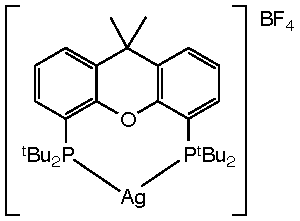
\includegraphics{../Structures/CtBuSilverBF4.pdf}
\end{center}
\end{structure}

%This reaction was carried out in the dark as silver chloride and the product are light sensitive.  Combined \fixme{CtBu ligand} (17 mg, 0.034 mmol) and silver chloride (5 mg, 0.035 mmol) in an NMR tube and dissolved in \ce{CDCl3}.  After 48 hours sonicated 10 x 5 mins, decanted the solution from the solid and vacced to dryness leaving a white powder.  \fixme{yield}

%Phosphorus
\Phosphorusintro{CDCl3}
\NMRAgP{27.6}{486.3}{561.1}
%Proton
\Protonintro{500}{CDCl3}
\NMRmultiplet{7.63-7.67}{4H, PC(Ar)C\emph{H}, PCCCC\emph{H}}
\NMRHH{7.29}{t}{7.7}{PC(Ar)CC\emph{H}}
\NMRsinglet{1.59}{C(bridge)C\emph{H\textsubscript{3}}}
\NMRmultiplet{1.39-1.42}{PCC\emph{H}\textsubscript{3}}
%Carbon
\Carbonintro{125}{CDCl3}
\NMRPC{154.9}{vt}{5.6}{\emph{C}O}
\NMRPC{133.5}{vt}{1.9}{PC(Ar)(\emph{C}H}
\NMRPC{133.5}{d}{5.8}{C(bridge)\emph{C}(Ar)}
\NMRsinglet{128.4}{PCCC\emph{C}H}
\NMRsinglet{123.8}{PC(Ar)C\emph{C}H}
\NMRsinglet{117.8}{P\emph{\emph{C}(Ar)}}
\NMRPC{35.6}{vtd}{5.3, 2.4}{\emph{C}(Bridge)}
\NMRPC{35.3}{\fixme{d,d,d?}}{4.8, 2.7, 7.6}{P\emph{C}\ce{CH3}}
\NMRPC{30.6}{\fixme{d,d,d?}}{5.3, 4.4, 6.5}{PC\emph{C}\ce{H3}}
\NMRsinglet{29.4}{C(bridge)\emph{C}\ce{H3}}
%Fluorine
\Fluorineintro{CDCl3}
\NMRsinglet{-152.0ppm}{\ce{BF4-}}

\fixme{Need to check and get all of the couplings}
\fixme{Make sure that all of the proton couplings around all of the rings have consistent PH or HH}
\fixme{Consider using numbering}
\fixme{check how on earth to write up all of the tBu couplings...}

%%%%%%%%
%PdCl2 StBu %
%%%%%%%%
%\newpage{}
%\subsection*{\emph{t}-Bu-thixantphospalladiumdichloride, 2020} \fixme{check name}
%\begin{structure}[h]
%\begin{center}
%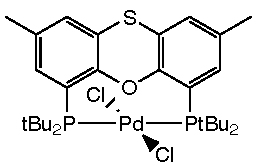
\includegraphics{../Structures/PdCl2(s(tBu)2)_complex.pdf}
%\end{center}
%\end{structure}

%\fixme{StBu ligand} (36 mg, 0.070 mmol) and \ce{[Pd(COD)Cl2]} (20 mg, 0.070 mmol) were combined in an NMR tube and dissolved in \ce{C6D6} and heated to 60\degC{} for 48 hours.  The solvent was removed in vacuo yielding the title compound as a dark red solid (37 mg, 77\%).

%Phosphorus
%\Phosphorusintro{C6D6}
%\NMRPsinglet{41.9}
%Proton
%\Protonintro{500}{C6D6}
%\NMRsinglet{7.17}{PC(Ar)\emph{H}},
%\NMRsinglet{7.15}{SCC\emph{H}}
%\NMRsinglet{2.33}{C(Ar)\ce{C\emph{H}3}}
%\NMRPH{1.59}{vt}{7.1}{PCC\emph{H}\textsubscript{3}}
%Carbon
%\Carbonintro{125}{CDCl3}
%\NMRPC{155.1}{vt}{4.8}{\emph{C}O}
%\NMRsinglet{134.4}{PC(Ar)\emph{C}H}
%\NMRPC{133.4}{vt}{\fixme{?}}{\emph{C}(Ar)\ce{CH3}}
%\NMRsinglet{130.4}{SC\emph{C}H})
%\NMRmultiplet{123.5}{P\emph{C}(Ar)}
%\NMRPC{123.1}{vt}{3.0}{\emph{C}S}
%\NMRPC{39.5}{vt}{5.8}{P\emph{C}C\ce{H3}}
%\NMRsinglet{31.2}{PC\emph{C}\ce{H3}}
%\NMRsinglet{20.7}{C(Ar)\emph{C}\ce{H3}}

%\fixme{IR, EA, 1H, 31P, 13C, MS}
%\fixme{Redraw complex with new parameters}
%\fixme{Check solvent}

\section{Platinum Complexes}
\label{section:experimental:platinum}

%%%%%%
% PtStBu %
%%%%%%

\subsection*{\emph{t}-Bu-Thixantphosplatinum}
\begin{structure}[h]
\begin{center}
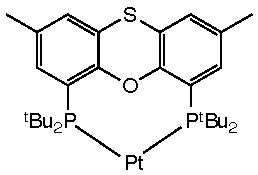
\includegraphics{../Structures/StBuPlatinum.pdf}
\end{center}
\end{structure}

\subsubsection{Starting from Pt(COD)2}
\subsubsection{Starting from Pt(nb)3}

\Phosphorusintro{C6D6}
\NMRPPt{78.6}{4809.5}
\Protonintro{600}{C6D6}
\NMRPH{7.32}{d}{1.8}{PC(Ar)C\emph{H}},
\NMRsinglet{6.87}{SCC\emph{H}},
\NMRsinglet{1.95}{C(Ar)\ce{C\emph{H}3}},
\NMRPH{1.52}{vt}{13.8}{PCC\emph{H}\textsubscript{3}}.
\Carbonintro{150}{C6D6}
\NMRPC{155.9}{vt}{10.4}{\emph{C}O}
\NMRsinglet{133.3}{PC(Ar)\emph{C}H}
\NMRPC{132.1}{vt}{5.2}{SCC\emph{C}(\ce{CH3})}
\NMRsinglet{128.8}{\emph{C}(Ar)\ce{CH3}}
\NMRPC{126.6}{vt}{28.9}{P\emph{C}(Ar)}
\NMRPC{126.1}{vt}{5.8}{\emph{C}S}
\NMRPC{37.8}{vt}{15}{P\emph{C}\ce{CH3}}
\NMRPC{31.7}{vt}{10.4}{PC\emph{C}\ce{H3}}
\NMRsinglet{20.5}{C(Ar)\emph{C}\ce{H3}}.
\fixme{IR, EA, MS}


%%%%%%%%
% PtStBu(nb) %
%%%%%%%%

\subsection*{\emph{t}-Bu-Thixantphosplatinumnorbornene}
\begin{structure}[h]
\begin{center}
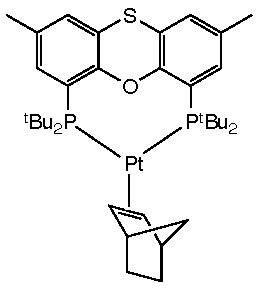
\includegraphics{../Structures/StBuPlatinumnorbornene.pdf}
\end{center}
\end{structure}

\Phosphorusintro{C6D6}
\NMRPPt{55.6}{3612}
\Protonintro{600}{C6D6}
\NMRsinglet{7.61}{PC(Ar)C\emph{H}},
\NMRsinglet{6.95}{SCC\emph{H}},
\NMRsinglet{3.12}{nb CH},
\NMRPtH{2.37}{bs}{1}{67.8}{nb =C\emph{H}},
\NMRsinglet{1.96}{C(Ar)\ce{C\emph{H}3}},
\NMRobscuredH{1.93}{COSY}{2H}{nb C\emph{H}\textsubscript{2}},
\NMRmultiplet{1.42-1.56}{PCC\emph{H}\textsubscript{3}},
\NMRobscuredH{1.32}{COSY}{3H}{nb C\emph{H}\textsubscript{2}, bridge \ce{CH2}},
\NMRHH{0.62}{d}{15.3}{1H, nb bridge \ce{CH2}}
\Carbonintro{150}{C6D6}
\NMRPC{158.9}{vt}{9.8}{\emph{C}O},
\NMRPtC{135.4}{s}{2}{26.6}{PC(Ar)\emph{C}H},
\NMRbsinglet{130.9}{\emph{C}(Ar)\ce{CH3}},
\NMRbsinglet{130.7}{SCC\emph{C}(\ce{CH3})},
\NMRPC{127.6}{vt}{5.8}{\emph{C}S},
\NMRbsinglet{125.9}{P\emph{C}(Ar)},
\NMRPtC{51.9}{bs}{1}{343.9}{nb =\emph{C}H},
\NMRsinglet{44.9}{nb \emph{C}H},
\NMRmultiplet{38.5}{P\emph{C}\ce{CH3}},
\NMRobscuredC{38.0-38.5}{HSQC}{nb bridge \emph{C}\ce{H2}},
\NMRbsinglet{31.7}{PC\emph{C}\ce{H3}},
\NMRPtC{31.4}{bs}{3}{61.4}{nb \emph{C}\ce{H2}},
\NMRsinglet{20.7}{C(Ar)\emph{C}\ce{H3}}.
\fixme{IR, EA, MS}

%%%%%%%%%
% PtStBuC2H4 %
%%%%%%%%%
\subsection*{\emph{t}-Bu-Thixantphosplatinumethene}
\begin{structure}[h]
\begin{center}
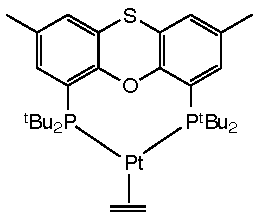
\includegraphics{../Structures/StBuPlatinumethene.pdf}
\end{center}
\end{structure}

\Phosphorusintro{C6D6}
\NMRPPt{55.7}{3899}
\Protonintro{600}{C6D6}
\NMRsinglet{7.63}{PC(Ar)C\emph{H}},
\NMRsinglet{6.96}{SCC\emph{H}},
\NMRPtH{2.50}{bs}{1}{59.5}{\ce{C=C-H2}},
\NMRsinglet{1.97}{C(Ar)\ce{C\emph{H}3}},
\NMRmultiplet{1.38-1.40}{PCC\emph{H}\textsubscript{3}},
\Carbonintro{150}{C6D6}
\NMRbsinglet{158.7}{\emph{C}O},
\NMRPtC{135.3}{s}{2}{29.5}{PC(Ar)\emph{C}H},
\NMRbsinglet{131.0}{\emph{C}(Ar)\ce{CH3}},
\NMRbsinglet{130.5}{SCC\emph{C}(\ce{CH3})},
\NMRPC{128.5}{vt}{5.8}{\emph{C}S},
\NMRbsinglet{125.7}{P\emph{C}(Ar)},
\NMRmultiplet{38.7}{P\emph{C}\ce{CH3}},
\NMRPtC{34.2}{bs}{1}{223.2}{\ce{C=C}}
\NMRbsinglet{31.6}{PC\emph{C}\ce{H3}},
\NMRsinglet{20.7}{C(Ar)\emph{C}\ce{H3}}.
\fixme{IR, EA, MS}

%%%%%%%
%PtStBuO2%
%%%%%%%
\subsection*{\emph{t}-Bu-Thixantphosplatinumdioxygen}
\begin{structure}[h]
\begin{center}
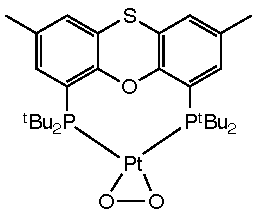
\includegraphics{../Structures/StBuPtO2.pdf}
\end{center}
\end{structure}

\Phosphorusintro{CD2Cl2}
\NMRPPt{38.4}{4488}
\Protonintro{600}{CD2Cl2}
\NMRcoupled{7.59}{dd}{5.9, 1.0}{a},
\NMRsinglet{7.32}{c},
\NMRsinglet{2.34}{g},
\NMRPH{1.43}{d}{14.4}{C(Ar)\ce{C\emph{H}3}},
\Carbonintro{125}{CD2Cl2}
\NMRbsinglet{156.6}{\emph{C}O},
\NMRPtC{133.8}{s}{2}{37.9}{PC(Ar)\emph{C}H},
\NMRPC{133.1}{d}{5.3}{\emph{C}(Ar)\ce{CH3}},
\NMRbsinglet{131.7}{SCC\emph{C}(\ce{CH3})},
\NMRsinglet{128.5}{\emph{C}S},
\NMRPC{119.3}{d}{27.8}{P\emph{C}(Ar)},
\NMRPC{39.3}{d}{23.5}{P\emph{C}\ce{CH3}},
\NMRPC{31.2}{d}{5.3}{PC\emph{C}\ce{H3}},
\NMRsinglet{21.2}{C(Ar)\emph{C}\ce{H3}}.
\fixme{IR, EA, MS}

\subsubsection{Starting from Pt(C2H4)}
\subsubsection{Starting from 14-electron}

%%%%%%%%
% Metallated  %
%%%%%%%%
\subsection*{Metallated complex}
\begin{structure}[h]
\begin{center}
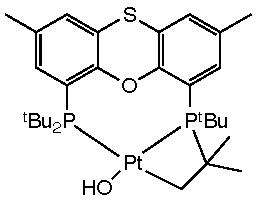
\includegraphics{../Structures/Metallated.pdf}
\end{center}
\end{structure}

\Phosphorusintro{CD2Cl2}
\NMRPtwoPt{38.17}{s}{1794}{\ce{P}-\textsuperscript{t}\ce{Bu2}}
\NMRPtwoPt{$-$49.63}{s}{3943}{\ce{PCCPt}}
\Protonintro{600}{CD2Cl2}
\NMRPH{7.60}{d}{3.8}{c2}
\NMRsinglet{7.25}{a1}
\NMRsinglet{7.16}{a2}
\NMRPH{6.95}{d}{6.5}{c1}
\NMRsinglet{2.34}{g1}
\NMRsinglet{2.32}{g2}
\NMRPH{1.71}{d}{12.9}{i3}
\NMRcoupled{1.41}{d}{15.9}{k}
\NMRcoupled{1.36}{d}{14.9}{l}
\NMRPH{1.34}{d}{13.2}{i2}
\NMRmultiplet{1.2-1.5, obscured}{m}
\NMRPH{1.03}{d}{15.0}{i1}
\Carbonintro{150}{CD2Cl2}
\NMRPC{157.1}{d}{9.0}{e2}
\NMRPC{153.9}{d}{4.3}{e1}
\NMRPC{134.2}{d}{3.2}{c2}
\NMRPC{133.8}{d}{6.3}{b1}
\NMRPC{133.4}{d}{3.2}{b2}
\NMRsinglet{132.8}{c1}
\NMRPC{130.5}{d}{1.6}{a1}
\NMRPC{129.6}{d}{1.6}{a2}
\NMRPC{128.5}{dd}{4.2, 1.6}{f1}
\NMRPC{124.0}{d}{4.3}{f2}
\NMRPC{121.3}{d}{13.8}{d2}
\NMRPC{116.6}{dd}{30.7, 1.6}{d1}
\NMRPC{46.7}{d}{37.6}
\NMRPC{40.8}{d}{10.1}{h2}
\NMRPC{36.8}{d}{8.0}{h3}
\NMRPC{36.0}{d}{22.3}{h1}
\NMRPC{33.2}{d}{5.8}{i3}
\NMRsinglet{32.6}{l}
\NMRPC{32.1}{dd}{10.1, 3.7}{k}
\NMRPC{31.3}{d}{5.3}{i2}
\NMRbsinglet{28.8}{i1}
\NMRsinglet{21.3}{g2}
\NMRsinglet{21.0}{g1}
\fixme{\NMRsinglet{15.7}{dd}{81.6, 35.5}{m}}
\fixme{IR, EA, MS}
\fixme{this data needs checked once it has been remade}

%%%%%%%
%PtStBuCl2%
%%%%%%%
\subsection*{\emph{trans}-(\emph{t}-Bu-Thixantphos)platinumdichloride}
\begin{structure}[h]
\begin{center}
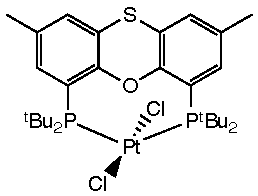
\includegraphics{../Structures/StBuPtCl2.pdf}
\end{center}
\end{structure}

\Phosphorusintro{C6D6}
\NMRPPt{32.9}{2700}
\Protonintro{500}{C6D6}
\NMRsinglet{7.11}{PC(Ar)C\emph{H}},
\NMRsinglet{6.98}{SCC\emph{H}},
\NMRsinglet{1.86}{C(Ar)\ce{C\emph{H}3}},
\NMRPH{1.71}{vt}{7.3}{PCC\emph{H}\textsubscript{3}},
\NMRbsinglet{1.56}{PCC\emph{H}\textsubscript{3}},
\Carbonintro{125}{C6D6}
\NMRPC{155.8}{vt}{\fixme{?}}{\emph{C}O},
\NMRsinglet{134.3}{PC(Ar)\emph{C}H},
\NMRPC{131.0}{vt}{3.4}{\emph{C}(Ar)\ce{CH3}},
\NMRsinglet{129.9}{SC\emph{C}C(\ce{CH3})},
\NMRPC{124.0}{P\emph{C}(Ar)},
\NMRPC{124.5}{vt}{\fixme{?}}{\emph{C}S},
\NMRsinglet{20.3}{C(Ar)\emph{C}\ce{H3}},
\NMRPC{39.7}{vt}{\fixme{?}}{PC\emph{C}\ce{H3}},
\NMRPC{38.8}{vt}{11.1}{PC\emph{C}\ce{H3}},
\NMRPC{32.8}{vt}{3.9}{P\emph{C}\ce{CH3}},
\NMRbsinglet{30.2}{P\emph{C}\ce{CH3}},
\fixme{IR, EA, MS}

%%%%%%%%%
%PtStBuCl PF6%
%%%%%%%%%
\subsection*{\emph{trans}-(\emph{t}-Bu-Thixantphos)platinumchloride hexafluorophosphate}
\begin{structure}[h]
\begin{center}
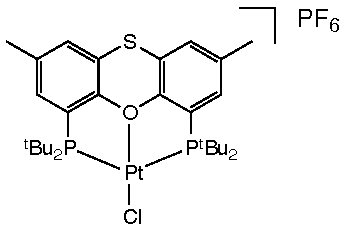
\includegraphics{../Structures/StBuPtClPF6.pdf}
\end{center}
\end{structure}

\Phosphorusintro{CD2Cl2}
\NMRPsinglet{46.4}
\NMRPF{-144.5}{septet}{710.5}{\emph{P}\ce{F6}}
\Protonintro{500}{CD2Cl2}
\NMRsinglet{7.41}{PC(Ar)C\emph{H}},
\NMRsinglet{7.11}{SCC\emph{H}},
\NMRsinglet{2.38}{C(Ar)\ce{C\emph{H}3}},
\NMRPH{1.55}{vt}{8.0}{PCC\emph{H}\textsubscript{3}},
\Carbonintro{125}{C6D6}
\NMRmultiplet{157.4}{\emph{C}O},
\NMRsinglet{138.9}{\emph{C}(Ar)\ce{CH3}},
\NMRsinglet{134.4}{PC(Ar)\emph{C}H},
\NMRsinglet{132.6}{SC\emph{C}C(\ce{CH3})},
\NMRmultiplet{119.8}{P\emph{C}(Ar)},
\NMRmultiplet{119.1}{\emph{C}S},
\NMRPC{40.0}{vt}{10.4}{P\emph{C}C\ce{H3}},
\NMRsinglet{30.1}{PC\emph{C}\ce{H3}},
\NMRsinglet{20.4}{C(Ar)\emph{C}\ce{H3}},
\Fluorineintro{CD2Cl2}
\NMRPF{-73.4}{d}{710.6}{P\emph{F}\textsubscript{6}}
\fixme{IR, EA, MS}

%%%%%%%%%
% PtStBuMe Cl %
%%%%%%%%%
\subsection*{\emph{trans}-(\emph{t}-Bu-Thixantphos)platinumchloride hexafluorophosphate}
\begin{structure}[h]
\begin{center}
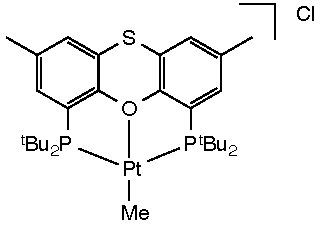
\includegraphics{../Structures/StBuPtMe.pdf}
\end{center}
\end{structure}

\Phosphorusintro{d6-acetone}
\NMRPsinglet{50.5}
\Protonintro{600}{d6-acetone}
\NMRPH{7.69}{d}{1.8}{PC(Ar)C\emph{H}},
\NMRPH{7.34}{d}{1.2}{SCC\emph{H}},
\NMRsinglet{2.42}{C(Ar)\ce{C\emph{H}3}},
\NMRPH{1.56}{vt}{15.6}{PCC\emph{H}\textsubscript{3}},
\NMRPH{1.94}{t}{5.5, \twoJPtH{}~=~97.4}{Pt-C\emph{H}\textsubscript{3}},
\Carbonintro{150}{d6-acetone}
\NMRPC{153.8}{vt}{10.3}{\emph{C}O},
\NMRPC{137.1}{vt}{6.3}{\emph{C}(Ar)\ce{CH3}},
\NMRsinglet{134.4}{PC(Ar)\emph{C}H},
\NMRsinglet{131.4}{SC\emph{C}C(\ce{CH3})},
\NMRPC{120.8}{vt}{31.8}{P\emph{C}(Ar)},
\NMRPC{118.2}{vt}{7.2}{\emph{C}S},
\NMRPC{38.8}{vt}{20.6}{P\emph{C}C\ce{H3}},
\NMRobscuredC{29.6}{\fixme{HSQC?}}{PC\emph{C}\ce{H3}},
\NMRsinglet{19.2}{C(Ar)\emph{C}\ce{H3}},
\NMRPC{-23.8}{t}{5.6, \oneJPtC{}~=~777.2}{Pt-\emph{C}\ce{H3}}
\fixme{IR, EA, MS}

\section{Palladium Complexes}
\label{section:experimental:palladium}

%%%%%%%%
% PdStBuCl2 %
%%%%%%%%
\subsection*{\emph{trans}-(\emph{t}-Bu-Thixantphos)palladiumdichloride}
\begin{structure}[h]
\begin{center}
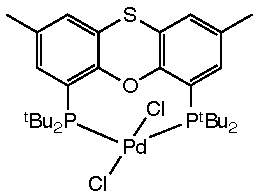
\includegraphics{../Structures/StBuPdCl2.pdf}
\end{center}
\end{structure}

\fixme{Check solvent}

\Phosphorusintro{C6D6}
\NMRPsinglet{41.9}
\Protonintro{500}{C6D6}
\NMRsinglet{7.17}{PC(Ar)C\emph{H}},
\NMRsinglet{7.15}{SCC\emph{H}},
\NMRsinglet{2.33}{C(Ar)\ce{C\emph{H}3}},
\NMRPH{1.59}{vt}{7.1}{PCC\emph{H}\textsubscript{3}},
\Carbonintro{125}{C6D6}
\NMRPC{155.1}{vt}{4.8}{\emph{C}O},
\NMRsinglet{134.4}{PC(Ar)\emph{C}H},
\NMRPC{133.4}{vt}{\fixme{?}}{\emph{C}(Ar)\ce{CH3}},
\NMRsinglet{130.4}{SC\emph{C}C(\ce{CH3})},
\NMRPC{123.5}{vt}{12.5}{P\emph{C}(Ar)},
\NMRsinglet{123.1}{\emph{C}S},
\NMRPC{39.5}{vt}{5.8}{P\emph{C}C\ce{H3}},
\NMRsinglet{31.2}{PC\emph{C}\ce{H3}},
\NMRsinglet{20.7}{C(Ar)\emph{C}\ce{H3}}
\fixme{IR, EA, MS}

%%%%%%%%
%PdCl2 SitBu %
%%%%%%%%
%\newpage{}
%2021
\subsection*{\emph{t}-Bu-Siixantphospalladiumdichloride} \fixme{check name}
\begin{structure}[h]
\begin{center}
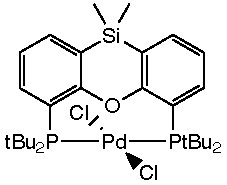
\includegraphics{../Structures/PdCl2(Si(tBu)2)_complex.pdf}
\end{center}
\end{structure}

Combined \fixme{StBu ligand} (12 mg, 0.023 mmol) and \ce{[Pd(COD)Cl2]} (7 mg, 0.025 mmol) in an \fixme{Youngs tube} and stirred at room temperature for 24 hours then 35\degC for a further 30 hours.  The solvent was removed in vacuo yielding a the title compound as a red solid \fixme{yield}.

\fixme{Include a structure}
%Phosphorus
\Phosphorusintro{CDCl3}
\NMRPsinglet{\fixme{get this value?}}
%Proton
\Protonintro{500}{CDCl3}
\NMRmultiplet{7.71}{PCC\emph{H}}
\NMRHH{7.68}{d}{7.1}{SiCC\emph{H}}
\NMRHH{7.33}{t}{7.3}{PCCC\emph{H}}
\NMRPH{1.60}{vt}{7.3}{PCC\emph{H}\textsubscript{3}}
\NMRsinglet{0.52}{SiC\emph{H}\textsubscript{3}}
%Carbon
\Carbonintro{125}{CDCl3}
\NMRPC{165.1}{vt}{\fixme{?}}{\emph{C}O}
\NMRsinglet{137.6}{PC\emph{C}H}
\NMRsinglet{136.9}{SiC\emph{C}H}
\NMRsinglet{124.9}{Si\emph{C}(Ar)}
\NMRsinglet{123.1}{PCC\emph{C}H}
\NMRPC{121.8}{vt}{13.4}{P\emph{C}(Ar)}
\NMRPC{39.6}{vt}{6.3}{P\emph{C}\ce{CH3}}
\NMRPC{31.1}{vt}{2.7}{PC\emph{C}\ce{H3}}
\NMRsinglet{-2.0}{Si\emph{C}\ce{H3}}.
\fixme{IR, mass spec, EA}
\fixme{Check the solvent}

%%%%%%%%%
% PdStBuClPF6%
%%%%%%%%%
\subsection*{\emph{trans}-(\emph{t}-Bu-Thixantphos)palladiumchloride hexafluorophosphate}
\begin{structure}[h]
\begin{center}
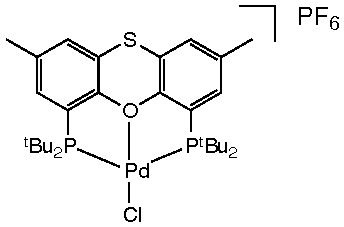
\includegraphics{../Structures/StBuPdClPF6.pdf}
\end{center}
\end{structure}

\fixme{Check solvent}

\Phosphorusintro{CD2Cl2}
\NMRPsinglet{56.4}
\NMRPF{-144.5}{septet}{710.5}{\emph{P}\ce{F6}}
\Protonintro{500}{CD2Cl2}
\NMRPH{7.36}{d}{2.0}{PC(Ar)C\emph{H}},
\NMRsinglet{7.15}{SCC\emph{H}},
\NMRsinglet{2.38}{C(Ar)\ce{C\emph{H}3}},
\NMRPH{1.58}{vt}{8.2}{PCC\emph{H}\textsubscript{3}},
\Carbonintro{125}{C6D6}
\NMRPC{154.86}{vt}{6.5}{\emph{C}O},
\NMRPC{138.3}{vt}{\fixme{?}}{\emph{C}(Ar)\ce{CH3}},
\NMRsinglet{134.6}{PC(Ar)\emph{C}H},
\NMRsinglet{132.6}{SC\emph{C}C(\ce{CH3})},
\NMRsinglet{119.1}{\emph{C}S},
\NMRPC{118.7}{vt}{10.8}{P\emph{C}(Ar)},
\NMRPC{40.2}{vt}{7.2}{P\emph{C}C\ce{H3}},
\NMRsinglet{30.1}{PC\emph{C}\ce{H3}},
\NMRsinglet{20.4}{C(Ar)\emph{C}\ce{H3}}
\Fluorineintro{CD2Cl2}
\NMRPF{-73.4}{d}{710.6}{P\emph{F}\textsubscript{6}}
\fixme{IR, EA, MS}

%%%%%%%%%
% PdStBuOAc2 %
%%%%%%%%%
\subsection*{\emph{trans}-(\emph{t}-Bu-Thixantphos)palladiumdiacetate}
\begin{structure}[h]
\begin{center}
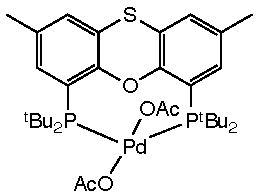
\includegraphics{../Structures/StBuPdOAc2.pdf}
\end{center}
\end{structure}

\Phosphorusintro{C6D6}
\NMRPsinglet{33.7}
\Protonintro{500}{C6D6}
\NMRPH{7.07}{d}{2.0}{PC(Ar)C\emph{H}},
\NMRsinglet{6.83}{SCC\emph{H}},
\NMRsinglet{1.89}{C(Ar)\ce{C\emph{H}3}},
\NMRbsinglet{1.42}{PCC\emph{H}\textsubscript{3}},
\fixme{Peak for acetates?}
\Carbonintro{125}{C6D6}
\NMRbsinglet{177.7}{O\emph{C}(O)\ce{CH3}}
\NMRPC{156.3}{vt}{8.4}{\emph{C}O},
\NMRPC{134.4}{d}{13.9}{PC(Ar)\emph{C}H},
\NMRsinglet{132.9}{\emph{C}(Ar)\ce{CH3}},
\NMRsinglet{129.9}{SC\emph{C}C(\ce{CH3})},
\NMRPC{123.5}{vt}{\fixme{?}}{\emph{C}S},
\NMRPC{120.3}{vt}{22.4}{P\emph{C}(Ar)},
\NMRPC{37.0}{vt}{10.2}{P\emph{C}C\ce{H3}},
\NMRbsinglet{30.3}{PC\emph{C}\ce{H3}},
\NMRbsinglet{24.3}{OC(O)\emph{C}\ce{H3}}
\NMRsinglet{20.3}{C(Ar)\emph{C}\ce{H3}}
\fixme{IR, EA, MS}

\newpage{}
\section{Things that need to be fixed or added for final thesis}
\begin{itemize}
\item{Check that negative sign is actually negative and not a hyphen or other type of dash}
\item{Check freezer temperature for recrystallisations}
\item{Include reaction between Pt(tBu-thixantphos)O2 and PTA}
\item{Include reaction between Pt(COD)2 and tBu-thixantphos}
\item{Make sure all captions have full stops}
\item{Check that bis and cis etc. are all italics or not as necessary}
\item{Double bonds look better in ce rather than as equals}
\item{Check that the correct measurements for virtual triplets are made}
\item{Correct my nmr stuff such that a is actually labelled correctly}
\item{Explain why my dichloride has two different tbu environments in the NMR}
\item{Note that tBu-xantphos is also used for the tBu on the backbone...}
\item{Should it be square-planar or square planar?}
\end{itemize}

\newpage{}
\section{Lab work that still needs to be done}
\begin{itemize}
\item{React dioxygen complex with CO2 to get a peroxycarbonate c.f. Goel1983b}
\item{See if reaction of the dioxygen complex with hydrogen results in the reduction to platinum(0), c.f. Sergeev2010}
\item{Repeat reaction of dioxygen complex with CO}
	\begin{itemize}
	\item{Get 13C shift of the metallated carbon}
	\item{Run long HSQC to low ppm to see if I can identify the protons}
	\item{Run VERY long 13C to try and see platinum satellites - very unlikely}
	\item{React metallated product with methane and hydrogen}
	\end{itemize}
\item{Run long carbon on 600 MHz of RhCl (4023) to find the missing carbon}
\item{Purifiy the StBu selenide then get and assign full set}
\item{Repeat reaction with Pt(C2H4)3 and StBu to in sealed tube to prevent oxidation and check that everything that is made is the ethene complex}
\item{Repeat reaction with Pt(COD)2 and StBu in a sealed NMR tube to ensure that no COD complex forms}
\item{Repeat reaction with Rh(COE)2Cl and StBu in acetone and see if the Rh(III) complex forms faster - check the NMR of 4037 to see any sign of complexed acetone}
\item{Complete reaction between Ir(COE)2Cl and StBu}
\item{React CtBu and SitBu with Pt(nb)3 as comparisons or sterics etc.}
\item{React PtMeStBu complex with PF6 to confirm the structure as without a chloride}
\item{Reduce PdCl complex in the air to form a palladium dioxygen complex look at 2009 before you do this}
\item{Get John to make Pd(nb)3 to react and form a palladium(0) complex}
\item{Calculate structure of Pt(POP)Me complex to see if an agostic is present}
\item{React C bridged ligand with Pt(nb)3}
\item{React ligand with RhCl3 to see if the degradation product is a RhCl3 complex}
\item{Purify and re-run full set on the StBu selenide - 4026}
\end{itemize}

\section{Lab work that would be nice to do}
\begin{itemize}
\item{VT NMR on all three protonated ligands}
	\begin{itemize}
	\item{Get coalescence temperatures as an indication of the amount of exchange that is occurring}
	\end{itemize}
\item{React 14-electron complex with silane and HCl to try and identify the unknown hydride that forms when reacting with Pt(COD)2 or Pt(nb)3}
\item{Palladium analogue of PtMe}
\item{Protonation of PtMe complex}
\end{itemize}

\newpage{}
\section{Home work that still needs to be done}
\begin{itemize}
\item{Update Olex2 on laptop}
\item{Get scifinder working on laptop}
\item{Get mercury working on laptop}
	\begin{itemize}
	\item{Find out how to measure backbone bending}
	\end{itemize}
\end{itemize}

\section{Desk work that still needs to be done}
\begin{itemize}
\item{Complete bite-angle calculations}
\item{Check for the VT that I did on the protonated ligand}
\item{Look up structures for Pt(P)2 on scifinder and CCD}
	\begin{itemize}
	\item{Check if there are any with diphosphines, van Leeuwens review suggested that there were not}
	\end{itemize}
\item{Check 600 MHz for a carbon on 4019 after 18/4}
\item{Check solubility of CO across different temperatures}
\item{Look at 4027 (oxidation of StBu) to try and find evidence of S oxidation}
\item{Look at VT on 4029 - dichloride complex}
\item{Fully assign 4031 (CtBu selnide?)}
\item{Assign IR stretches}
	\begin{itemize}
	\item{It may be necessary to compare with calculated IRs}
	\end{itemize}
\item{Check the integrals for nb, ethene and COD complexes to go into thesis}
\item{ORTEP diagrams of crystal structures}
\item{Update the synthesis books}
\item{Read paper from John on dioxygen reactivity}
\item{Read up on iridium hydride metallation stuff, see Kranenburg1995 for an unusual Rh complex}
\item{Read Mora2008 to get ideas for catalysis}
\item{Read Casey1990 for full description of bite-angle stuff}
\item{Read up on through space NMR coupling with relation to the protonated ligands - ask Robin?}
\item{Update lab book}
\item{Get mestranova NMR stuff for the VT on the dichloride (4009?) that I did}
\end{itemize}

%\subsection*{2,4-Di(carbomethoxy)-1,5-bis(\emph{p}-dimethylaminophenyl)-penta-1,4-dien-3-one}

%\begin{structure}
%\begin{center}
%\includegraphics[scale=1.2]{structures/dba436}
%\end{center}
%\end{structure}


%\noindent Dimethyl 1,3-acetonedicarboxylate (3.5~g, 0.02 mol), \textit{p}-di\-methy\-lamino\-benz\-aldehyde (6.0~g, 0.04 mol), piperidine (0.45~\cm, 4.6~mmol) and glacial acetic acid (0.30~\cm, 5.2~mmol) were combined in benzene (60~\cm) in a 250~\cm{} round bottom flask in the air.  The flask was equipped with a Dean-Stark trap to measure the volume of water being eliminated during the course of the reaction.  The trap was in turn equipped with a condenser, and the reaction mixture was heated under reflux for 1 day.  About 0.7~\cm{} of water were collected in the Dean-Stark trap indicating that the reaction was complete.  The solvent was removed \textit{in vacuo} to yield a dark red oil.  The oil was washed with petroleum ether several times then taken up in benzene.  The mixture was stirred at room temperature for several hours during which yellow crystalline solid precipitated out as the oil slowly dissolved.  The solid was filtered, washed with benzene and dried in the air
%(7.5~g, 86\%); 
%mp 124.5-124.8\degC{} (from benzene);
%(Found: C, 69.2; H, 6.5; N, 6.4. \ce{C25H28N2O5} requires C, 68.8; H, 6.5; N, 6.4\%);
%\numax(KBr)/\percm{} 1732, 1719, 1701, 1693, 1572, 1526, 1373, 1189 and 1158;  
%\dH(300~MHz; \ce{C6D6}; \ce{Me4Si}) 
%2.18 (6 H, s, \ce{NMe2}), 
%2.19 (6 H, s, \ce{NMe2}), 
%3.43 (3 H, s, OMe), 
%3.69 (3 H, s, OMe), 
%6.12 (2 H, d, \JHH{} 9.0, \textit{m}-H), 
%6.23 (2 H, d, \JHH{} 9.0, \textit{m}-H), 
%7.31 (2 H, d, \JHH{} 9.0, \textit{o}-H), 
%7.62 (2 H, d, \JHH{} 9.0, \textit{o}-H), 
%7.88 (1 H, s, CH=CH) and 
%8.32 (1 H, s, CH=CH);  
%\dC(75~MHz; \ce{C6D6}; \ce{Me4Si}) 
%39.15 (2 C, s, \ce{NMe2}), 
%39.17 (2 C, s, \ce{NMe2}), 
%51.8 (1 C, s, OMe), 
%52.0 (1 C, s, OMe), 
%111.8 (1 C, s, \textit{m}-\ce{C6H4}), 
%112.1 (1 C, s, \textit{m}-\ce{C6H4}), 
%120.9 (2 C, s, \ce{C6H4}), 
%121.2 (2 C, s, \ce{C6H4}), 
%132.5 (2 C, s, \textit{o}-\ce{C6H4}), 
%133.2 (2 C, s, \textit{o}-\ce{C6H4}), 
%143.7 (1 C, s, \textit{p}-\ce{C6H4}), 
%143.9 (1 C, s, \textit{p}-\ce{C6H4}), 
%166.5 (1 C, s, COO), 
%169.3 (1 C, s, COO) and 
%193.8 (1 C, s, CO);
%\textit{m/z} (ESI) 459.1000 (\MplusNa. \ce{C25H28N2O5Na} requires 459.1896).